
% This LaTeX was auto-generated from MATLAB code.
% To make changes, update the MATLAB code and republish this document.

\documentclass{article}
\usepackage{graphicx}
\usepackage{color}

\sloppy
\definecolor{lightgray}{gray}{0.5}
\setlength{\parindent}{0pt}

\begin{document}

    
    \begin{verbatim}
sig_x = 1;
sig_xy = -.5;
sig_y = 3;
mu_x = 1;
mu_y = 0;

X = randn();
Y = randn();

for n=1:20000
    mu = mu_x + sig_xy*inv(sig_y)*(Y(1)-mu_y);
    sig = sig_x-sig_xy*inv(sig_y)*sig_xy;
    X(n+1) = normrnd(mu,sig);

    mu = mu_y + sig_xy*inv(sig_x)*(X(n+1)-mu_x);
    sig = sig_y-sig_xy*inv(sig_x)*sig_xy;
    Y(n+1) = normrnd(mu,sig);
end

figure
hold on
histogram(X(1000:20000),'Normalization','pdf')
plot(-10:.1:10,normpdf(-10:.1:10,1,1))
title('p(x1)')

figure
hold on
histogram(Y(1000:20000),'Normalization','pdf')
plot(-10:.1:10,normpdf(-10:.1:10,0,3))
title('p(x2)')
\end{verbatim}

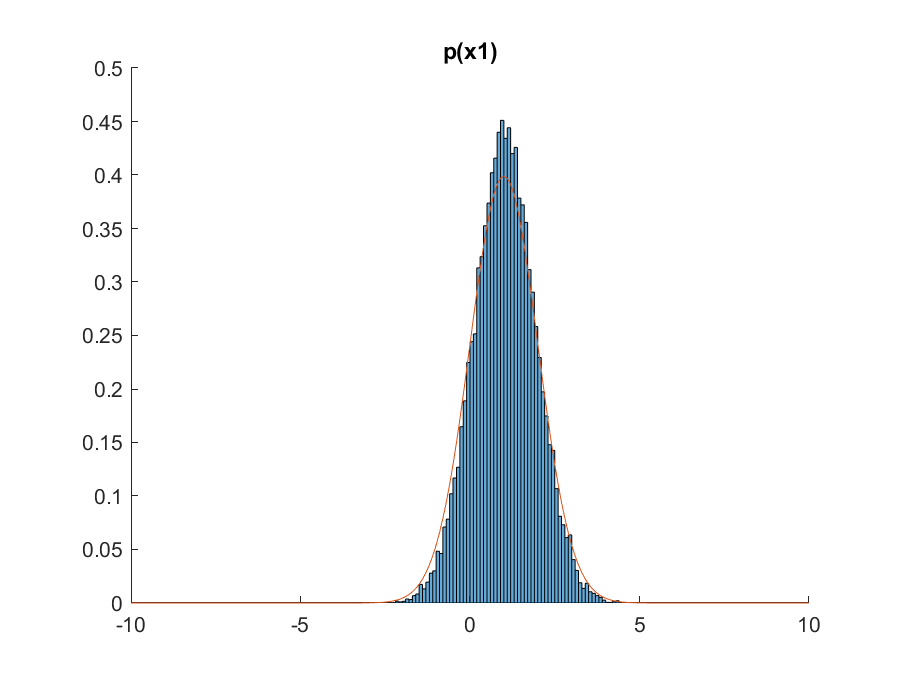
\includegraphics [width=4in]{hw5p2_01.eps}

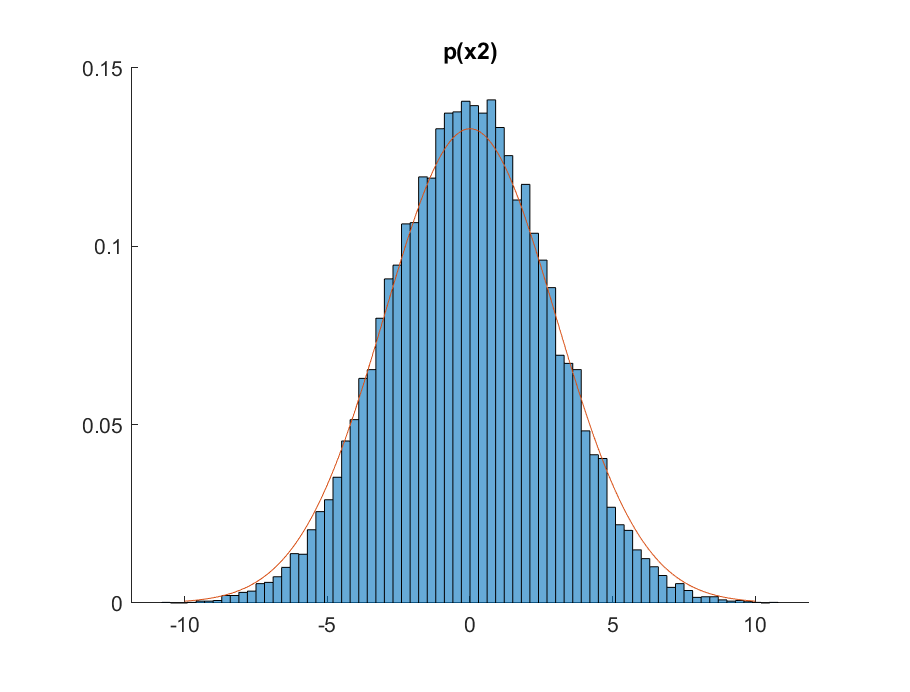
\includegraphics [width=4in]{hw5p2_02.eps}



\end{document}
    
